\documentclass[a4paper,12pt]{article}
%%%%%%%%%%%%%%%%%%%%%%%%%%%%%%%%%%%%%%%%%%%%%%%%%%%%%%%%%%%%%%%%%%%%%%%%%%%%%%%%%%%%%%%%%%%%%%%%%%%%%%%%%%%%%%%%%%%%%%%%%%%%%%%%%%%%%%%%%%%%%%%%%%%%%%%%%%%%%%%%%%%%%%%%%%%%%%%%%%%%%%%%%%%%%%%%%%%%%%%%%%%%%%%%%%%%%%%%%%%%%%%%%%%%%%%%%%%%%%%%%%%%%%%%%%%%
\usepackage{eurosym}
\usepackage{vmargin}
\usepackage{amsmath}
\usepackage{framed}
\usepackage{multicol}
\usepackage{graphics}
\usepackage{epsfig}
\usepackage{subfigure}
\usepackage{enumerate}
\usepackage{fancyhdr}

\setcounter{MaxMatrixCols}{10}
%TCIDATA{OutputFilter=LATEX.DLL}
%TCIDATA{Version=5.00.0.2570}
%TCIDATA{<META NAME="SaveForMode"CONTENT="1">}
%TCIDATA{LastRevised=Wednesday, February 23, 201113:24:34}
%TCIDATA{<META NAME="GraphicsSave" CONTENT="32">}
%TCIDATA{Language=American English}

\pagestyle{fancy}
\setmarginsrb{20mm}{0mm}{20mm}{25mm}{12mm}{11mm}{0mm}{11mm}
\lhead{MathsResource} \chead{Linear Regression Models} \rhead{Tutorial Sheet} %\input{tcilatex}
\begin{document}




\begin{enumerate}

\item Discuss the statement “Correlation does not imply causation” within the context of data analysis.

\item A survey was conducted in 9 areas of the USA to investigate the relationship between divorce rate (y) and residential mobility (x). Divorce rates in the annual number per 1000 in the population and the residential mobility is measured by the percentage of the population that moved house in the last five years.

\begin{center}
\begin{tabular}{|c|c|c|c|c|c|c|c|c|c|}
	\hline
	Area & 1 & 2 & 3 & 4 & 5 & 6 & 7 & 8 & 9  \\
	x & 40 & 38 & 46 & 49 & 47 & 43 & 51 & 57 & 55\\
	y & 3.9 & 3.4 & 5.2 & 4.8 & 5.6 & 5.8 & 6.6 & 7.6 & 5.8\\
	\hline
\end{tabular}
\end{center}

\begin{enumerate}[(a)]
	\item Check that the following statements are correct.
	
	\begin{itemize}
		\item sum of x data = 426
		\item sum of squares of x data = 20494
		\item sum of y data = 48.7
		\item sum of squares of y data = 276.81
		\item sum of products of x and y data = 2361
	\end{itemize}
	
	\item Derive the estimates for the slope and intercept of the regression line.
	\item Estimate the divorce rate for areas that has a residential mobility of 39 and 60 respectively.
	\item Which of these estimates is likely to be more accurate? Why?
	
\end{enumerate}

%===============================================================%

\item An insurance company is interested in estimating the relationship between the rebuild cost of a detached house and the size of the house measured in square metres. Rebuild quotations were provided for a sample of 14 detached houses. The following data with summary measures were obtained:

\begin{center}
 \begin{tabular}{|c|c|c|c|c|c|c|c|c|c|c|c|c|c|c|}
	\hline
House size (x)  & 70 &  83 & 74 & 93 &  140 &  85 & 114 & 95 & 100 & 111 & 140 & 161 \\ 

Rebuild cost (y) & 80 & 90 & 100 & 110 & 320 & 150 & 160 & 180 & 200 & 250 & 270 & 320 \\
	\hline
\end{tabular}   
\end{center}
%%%%%%%%%%%%%%%%%%%%%%%%%%%%%%%%%%%%%%%%
\begin{enumerate}[(a)]
\item Describe the relationship between house size and rebuild cost using the scatter plot below.
\item Compute the Pearson correlation coefficient. Interpret this value.
\item Determine the least squares regression equation. Interpret the meaning of the slope of the regression line. 
\item Use the regression line to estimate the rebuild cost for a house sized 120 square metres.
\item Using the 5\% significance level, test the significance of the slope. Interpret the result.
\item Calculate and interpret the coefficient of determination.
\item What assumptions should a regression model satisfy? How can these assumptions be checked?
\end{enumerate}

\item An experiment was conducted to study the relationship between baking temperature $X$ (in units of 10 degrees Fahrenheit) and yield $Y$ (as percentage) of popular cake mix. Fourteen observations were made giving the following results.

%Temp 10 10.5 11 11.5 12 15 17 19 20 21 23 25 27 30

%Yield 21.2 19.9 22.5 23.7 25 30.3 36.1 38.6 41.5 42.7 45 50 53.9 62.1



\begin{center}
	\begin{tabular}{|c||c|c|c|c|c|c|c|}
		\hline
		Specimen & 1 & 2 & 3 & 4 & 5 & 6 & 7 \\ \hline
		\hline
		Temp &  10.00 & 10.50 & 11.00 & 11.50 & 12.00 & 15.00 & 17.00 \\ \hline 
		Yield &  29.830&  26.370 & 30.325 &36.100 &33.410 &36.335 & 40.655 \\ \hline 
		\hline\hline
		Specimen & 8 & 9 & 10 & 11 & 12 & 13 & 14 \\  \hline
		Temp &  19.00 & 20.00 & 21.00 & 23.00 & 25.00 & 27.00 & 30.00 \\ \hline
		Yield &  39.475& 44.555&  42.015 & 47.795 & 45.560&  51.045 & 47.900 \\ \hline 
		\hline
	\end{tabular}
\end{center}

\begin{multicols}{3}
	\begin{itemize}
		\item $S_{XX} = 570.5$
		\item $S_{YY} =  751.1525$
		\item $S_{XY} = 613.27$
		\item $\bar{X} = 18$
		\item $\bar{Y} = 39.383$
	\end{itemize}
\end{multicols}
\medskip

\begin{figure}
\centering
\includegraphics[width=0.99\linewidth]{images/MA4603-Regression-Repeat}
\caption{}
\label{fig:ma4603-regression-repeat}
\end{figure}
\medskip
\begin{enumerate}[(i)]
	
	\item (1 Mark) Using the scatter plot, describe the relationship between the yield (Y) and the baking temperature (X).
	
	
	
	
	
	\item (3 Marks) Calculate the correlation coefficient. Interpret your answer.
	\item (4 Marks) Calculate the equation of the least squares regression line and interpret the value of the slope.
	\item (2 Marks) Using this regression model, estimate the yield when the baking temperature is 16 degrees.
	%		\item (2 Marks) How much of the variation in yield is explained by fitting the regression line?
\end{enumerate}
\smallskip


%======================================%

\item An experiment was conducted to study the relationship between baking temperature x (in units of 10 degrees Farenheit) and yield y (as percentage) of popular cake mix. Fourteen observations were made giving the following results.

%Temp 10 10.5 11 11.5 12 15 17 19 20 21 23 25 27 30

%Yield 21.2 19.9 22.5 23.7 25 30.3 36.1 38.6 41.5 42.7 45 50 53.9 62.1



\begin{center}
	\begin{tabular}{|c||c|c|c|c|c|c|c|}
		\hline
		Specimen & 1 & 2 & 3 & 4 & 5 & 6 & 7 \\ \hline
		\hline
		Temp &  10.00 & 10.50 & 11.00 & 11.50 & 12.00 & 15.00 & 17.00 \\ \hline 
		Yield &  59.830&  58.370 & 60.325 &72.100 &66.410 &72.335 & 80.655 \\ \hline 
		\hline\hline
		Specimen & 8 & 9 & 10 & 11 & 12 & 13 & 14 \\  \hline
		Temp &  19.00 & 20.00 & 21.00 & 23.00 & 25.00 & 27.00 & 30.00 \\ \hline
		Yield &  78.475& 88.555&  84.015 & 94.795 & 90.560&  102.045 & 98.100 \\ \hline 
		\hline
	\end{tabular}
\end{center}

\begin{multicols}{3}
	\begin{itemize}
		\item $n=14$
		\item $S_{XX} = 570.5$
		\item $S_{YY} =  751.1525$
		\item $S_{XY} = 613.27$
		\item $\bar{X} = 18$
		\item $\bar{Y} = 39.383$
	\end{itemize}
\end{multicols}

\begin{figure}[h!]
	\centering
	\includegraphics[width=0.99\linewidth]{images/MA4505RegressionPlot}
\end{figure}
\medskip
\begin{enumerate}[(a)]
	\item Using the scatter plot, describe the relationship between the yield (Y) and the baking temperature (X).
	\item Calculate the correlation coefficient. Interpret your answer.
	\item Calculate the equation of the least squares regression line and interpret the value of the slope.
	\item Using this regression model, estimate the yield when the baking temperature is 16 degrees.
	\item How much of the variation in yield is explained by fitting the regression line?
\end{enumerate} % End of Last Part of Q5



\item A fire insurance company wants to relate the amount of fire damage in major residential fires to the distance between the residence and the nearest fire station. The study is to be conducted in a large suburb of a major city; a sample of 15 recent fires in this suburb is selected. The amount of damage (thousands of pounds) and the distance (in Kilometers) between the fire and the nearest station are recorded for each fire.

\begin{center}
\begin{tabular}{|c|c|c|c|c|c|}
  \hline
Incident	&	Distance (X) 	&	Fire Damage (Y)   	&	Incident	&	Distance (X) 	& Fire Damage (Y)   		 \\
1	&	3.4	&	21	&	9	&	2.6	&	15	\\
2	&	1.8	&	13	&	10	&	4.3	&	26	\\
3	&	4.6	&	26	&	11	&	2.1	&	19	\\
4	&	2.3	&	18	&	12	&	1.1	&	12	\\
5	&	3.1	&	23	&	13	&	6.1	&	38	\\
6	&	5.5	&	31	&	14	&	4.8	&	31	\\
7	&	0.7	&	9	&	15	&	3.8	&	21	\\
8	&	3	&	17	&		&		&		\\

  \hline
\end{tabular}



\begin{tabular}{lll}
  $\sum X = 49.2$ & $\sum Y = 320$ & $\sum XY = 1219.2$ \\
  $\sum X^2 = 196.16$ & $\sum Y^2 = 7722$ &  \\
 \end{tabular}
 \end{center}


\begin{enumerate}[(a)]
	\item Using the scatter plot, describe the relationship between the yield (Y) and the baking temperature (X).
	\item Calculate the correlation coefficient. Interpret your answer.
	\item Calculate the equation of the least squares regression line and interpret the value of the slope.
\item Find the equation of the regression line and plot the regression line on the scatter  diagram. Interpret the equation. 	
\item Using a significance level of $\alpha = 0.05$, test the claim that there is no linear correlation between distance and fire damage. 		
\end{enumerate}

\item 
% Correlation and Simple Linear Regression
% Non Parametric Procedures

A wood scientist wanted to establish if there was a relationship between the adhesive strength of laminated wood and the dwell time in press machine. A random sample of 9 different times and their corresponding adhesive strengths in pounds per square inch (PSI) were recorded as follows:

\begin{center}
\begin{tabular}{|c|c|c|}

  \hline
Sample &Time (Mins) & Pull Strength (PSI) \\
 & (X)  &  (Y)\\ \hline
1& 5.0& 3.5 \\
2& 4.8& 3.3\\
3& 5.6& 3.9\\
4& 4.3& 2.7\\
5& 4.2& 3.2\\
6& 5.4& 4.1\\
7& 5.5& 4.3\\
8& 4.0& 2.8\\
9& 4.7& 3.7\\
  \hline
\end{tabular}
\bigskip

\begin{tabular}{lll}
  $\sum X = 43.5$ & $\sum Y = 31.5$ & $\sum XY = 154.61$ \\
  $\sum X^2 = 213.03$ & $\sum Y^2 = 112.71$ &  \\
 \end{tabular}
 \end{center}
\begin{enumerate}[(a)]
\item Draw a scatter-plot and comment on its features.
\item Calculate the correlation coefficient. Interpret your answer.
\item Calculate the equation of the least squares regression line and interpret the value of the slope.
\item Using this regression model, estimate the adhesive strength for a piece of wood that has been in the press machine for 7 minutes.
\item Is such an estimate reliable? Briefly explain why.
\end{enumerate}

\item 
% Correlation and Simple Linear Regression
% Non Parametric Procedures
The following scatter-plot illustrates the relationship between the period of a pendulum in seconds and its length in metres (for 13 different lengths of the pendulum).

% \begin{center}
% 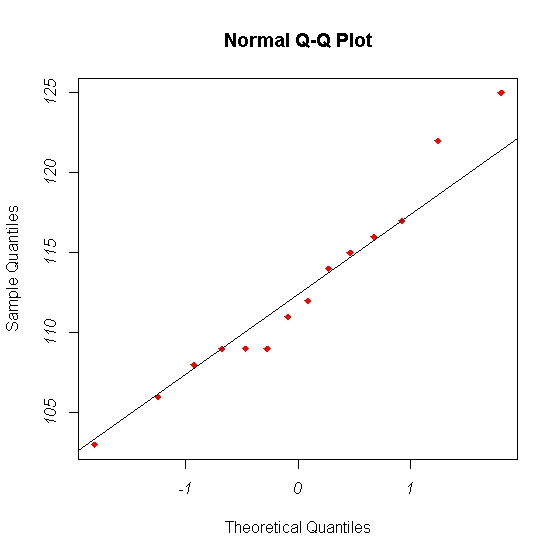
\includegraphics[scale=0.55]{images/Q5examQQplot.jpeg}
% \end{center}

\begin{center}
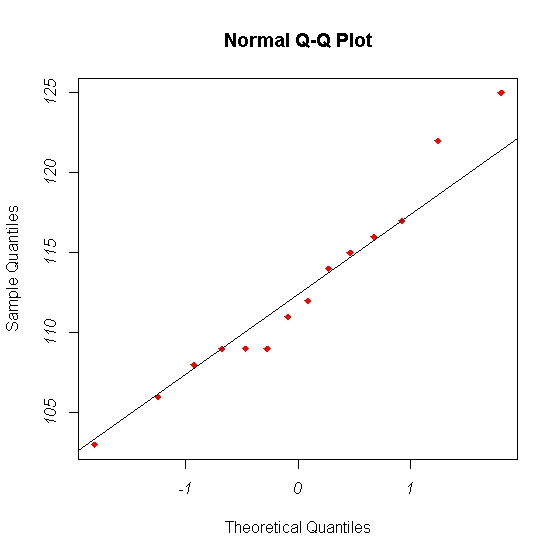
\includegraphics[scale=0.55]{images/Q5examQQplot.jpeg}
\end{center}
Use the following statistics to answer the following questions

\begin{center}
\begin{tabular}{lll}
  $\sum X = 43.5$ & $\sum Y = 31.5$ & $\sum XY = 3.068$ \\
  $\sum X^2 = 213.03$ & $\sum Y^2 = 112.71$ &  \\
 \end{tabular}
 \end{center}
 
 \begin{enumerate}[(a)]
     \item Calculate the equation of the least squares regression line and interpret the value of the slope.
\item Using this regression model, estimate the period of a pendulum of length 4m.
\item Briefly explain why this estimate is not reliable.
(2 marks)
 \end{enumerate}


\item The diameter at breast height (DBH) is a standard method of expressing the diameter of the trunk or bole of a standing tree. The DBH is one of the most common forestry measurements (\textit{``Dendrometrics"}). Researchers at a forestry company wish to develop a predictive model that would efficiently estimate the height of a tree (measured in metres) based on corresponding DBH value, measured in centimetres. 

Accurate measurements were taken from 200 randomly selected trees in the forestry company's plantation. These sets of measurements are depicted in the scatter plot on the next page. You are also given the following information: 
\begin{multicols}{3}
\begin{itemize}
\item $S_{XX}$ = 19,990
\item $S_{YY}$ = 3,680.50
\item $S_{XY}$ = 7,090.50
\item $\Sigma X$ = 5,190
\item $\Sigma Y$ = 3,692
\end{itemize}
\end{multicols}

 \begin{figure}[h!]
	\centering
	\includegraphics[width=0.89\linewidth]{images/Trees}
 \end{figure}
\smallskip
\begin{enumerate}[(a)]
	\item (2 Marks) Using the scatter plot, describe the relationship between the heights of the trees and the diameters at breast height (DBH).
	\item (3 Marks) Calculate the Pearson correlation coefficient. Interpret your answer.
	\item (4 Marks) Calculate the equation of the least squares regression line and interpret the value of the slope.
	\item (1 Marks) Using this regression model, estimate the tree height when the DBH is 20 centimetres. 
	\item (2 Marks) How much of the variation in yield is explained by fitting the regression line?
	
 \item Compute the Pearson Correlation Coefficient. Interpret this value.
 \item Determine the least squares regression equation. Interpret the meaning of the slope of the regression line.
\end{enumerate}


\end{enumerate}
\end{document}

